\documentclass[11pt]{article}
\usepackage[margin=1in]{geometry}
\usepackage[T1]{fontenc}
\usepackage{newtxtext,newtxmath}
\usepackage{microtype}
\usepackage{setspace}\setstretch{1.1}
\usepackage{parskip}
\usepackage{graphicx}
\usepackage{booktabs}
\usepackage{tabularx}
\usepackage{xcolor}
\usepackage{caption}
\usepackage{float}
\usepackage{enumitem}
\usepackage{titlesec}
\usepackage{fancyhdr}
\usepackage[hidelinks]{hyperref}
\usepackage[style=authoryear,backend=biber,maxcitenames=2,uniquename=false,uniquelist=false,useprefix=true]{biblatex}
\addbibresource{refs.bib}

\definecolor{oxide}{HTML}{8C3A1E}
\definecolor{ink2}{HTML}{52564E}
\titleformat{\section}{\large\bfseries}{\thesection}{0.8em}{}
\titleformat{\subsection}{\normalsize\bfseries}{\thesubsection}{0.8em}{}
\captionsetup{labelfont=bf,font=small,justification=raggedright,singlelinecheck=false}
\captionsetup[figure]{name=Exhibit}
\captionsetup[table]{name=Exhibit}
\renewcommand{\thetable}{\arabic{table}}
\makeatletter\let\c@table\c@figure\makeatother
\setlist{itemsep=2pt,topsep=4pt}
\pagestyle{fancy}\fancyhf{}
\renewcommand{\headrulewidth}{0pt}
\fancyfoot[L]{\footnotesize\color{ink2}Fuel Lockstep}
\fancyfoot[R]{\footnotesize\color{ink2}\thepage}

% Generated by scripts/export_numbers.py. Do not edit.
\newcommand{\hkDays}{2,373}
\newcommand{\hkStart}{30 April 2020}
\newcommand{\hkShareEqual}{87.6}
\newcommand{\hkEpisodes}{143}
\newcommand{\hkEpisodesUp}{110}
\newcommand{\hkEpisodesDown}{33}
\newcommand{\hkShareFullWeek}{90}
\newcommand{\hkShareSameDay}{1.4}
\newcommand{\hkShareSameSize}{83}
\newcommand{\hkMedianLag}{2}
\newcommand{\hkSizeUp}{0.20}
\newcommand{\hkSizeDown}{0.10}
\newcommand{\hkLeadShell}{37}
\newcommand{\hkLeadEsso}{17}
\newcommand{\hkLeadCaltex}{12}
\newcommand{\hkLeadSingle}{67}
\newcommand{\hkEqualTwentyThree}{96}
\newcommand{\hkEqualTwentySix}{78}
\newcommand{\hkUpTwentyThreeFour}{17}
\newcommand{\hkDownTwentyThreeFour}{0}
\newcommand{\postedFirst}{17.55}
\newcommand{\postedLast}{30.49}
\newcommand{\importFirst}{2.73}
\newcommand{\importLast}{5.40}
\newcommand{\marginFirst}{8.76}
\newcommand{\marginLast}{19.03}
\newcommand{\marginEnd}{2026-08}
\newcommand{\spanPostedFrom}{23.09}
\newcommand{\spanPostedTo}{28.89}
\newcommand{\spanImportFrom}{5.23}
\newcommand{\spanImportTo}{4.29}
\newcommand{\hkTrendYear}{2.08}
\newcommand{\perthStations}{419}
\newcommand{\perthRange}{38}
\newcommand{\perthIqr}{6}
\newcommand{\perthModal}{23}
\newcommand{\perthTue}{155.9}
\newcommand{\perthWed}{187.1}
\newcommand{\perthBrandRange}{10.4}
\newcommand{\hkUnchangedWeeks}{66}
\newcommand{\laUnchangedWeeks}{0.9}
\newcommand{\perthUnchangedWeeks}{16}
\newcommand{\hkRiseZero}{30}
\newcommand{\hkFallZero}{7}
\newcommand{\hkRiseFour}{67}
\newcommand{\hkFallFour}{39}
\newcommand{\hkAsymP}{0.009}
\newcommand{\hkWeeks}{334}
\newcommand{\laRiseZero}{53}
\newcommand{\laFallZero}{23}
\newcommand{\laRiseFour}{86}
\newcommand{\laFallFour}{85}
\newcommand{\laAsymP}{0.028}
\newcommand{\laWeeks}{334}
\newcommand{\perthRiseZero}{35}
\newcommand{\perthFallZero}{3}
\newcommand{\perthRiseFour}{95}
\newcommand{\perthFallFour}{104}
\newcommand{\perthAsymP}{0.280}
\newcommand{\perthWeeks}{347}
\newcommand{\discDays}{119}
\newcommand{\discFirst}{23 November 2020}
\newcommand{\discLast}{20 July 2026}
\newcommand{\discMaxFirst}{3.50}
\newcommand{\discMaxLast}{7.00}
\newcommand{\discNetMinFirst}{13.99}
\newcommand{\discNetMinLast}{25.04}
\newcommand{\discPumpFirst}{17.49}
\newcommand{\discPumpLast}{32.04}
\newcommand{\netMarginFirst}{6.74}
\newcommand{\postedMarginFirst}{9.19}
\newcommand{\netMeanFirst}{16.74}
\newcommand{\discMeanFirst}{2.44}
\newcommand{\netMarginLast}{13.11}
\newcommand{\postedMarginLast}{18.64}
\newcommand{\netMeanLast}{24.09}
\newcommand{\discMeanLast}{5.52}

\newcommand{\hk}{HK\$}

\begin{document}

\begin{titlepage}
\vspace*{1.2in}
{\footnotesize\color{ink2}\MakeUppercase{Retail fuel, Hong Kong}}\par\vspace{8pt}
{\LARGE\bfseries Lockstep at the pump\par}\vspace{6pt}
{\large Six years of parallel petrol pricing in Hong Kong, with Los Angeles and Perth as benchmarks\par}
\vspace{28pt}
{\normalsize Yiu-Hon Jeremy Lee\par}
{\small\color{ink2}October 2026\par}
\vfill
{\small\color{ink2}Code, data and every number in this paper: \url{https://github.com/lyhjeremy/fuel-lockstep}. Each figure in the text is generated from the analysis outputs by \texttt{scripts/export\_numbers.py}.\par}
\end{titlepage}

\section*{Executive summary}

Hong Kong's five petrol retailers (Caltex, Esso, PetroChina, Shell and Sinopec) almost always post the same pump price. This paper asks whether that pattern is what a small market with common costs would produce, or whether it shows features that costs do not explain. It uses \hkDays{} days of brand-level posted prices from the Consumer Council (\hkStart{} to October 2026), Hong Kong's monthly import price of petrol, and two comparison markets with many independent sellers: Los Angeles (weekly EIA retail and spot prices) and Perth (the price at every metropolitan station, every day, from FuelWatch).

\begin{itemize}
\item \textbf{Alignment is near total but not instantaneous.} The five brands posted the same Standard price on \hkShareEqual\% of days. Of \hkEpisodes{} price changes, all five brands matched within a week in \hkShareFullWeek\% of cases, usually within \hkMedianLag{} days, and by an identical amount in \hkShareSameSize\% of those. All five moved on the same day in only \hkShareSameDay\% of cases. One brand moves, the others follow.
\item \textbf{Shell leads most often.} Of the \hkLeadSingle{} changes started by a single brand, Shell started \hkLeadShell, Esso \hkLeadEsso{} and Caltex \hkLeadCaltex.
\item \textbf{Prices rise far more often than they fall.} \hkEpisodesUp{} changes were increases and \hkEpisodesDown{} were cuts. In 2023 and 2024 there were \hkUpTwentyThreeFour{} increases and \hkDownTwentyThreeFour{} cuts.
\item \textbf{The margin over import cost and duty roughly doubled, before and after discounts.} On the posted price it averaged \hk\marginFirst{} a litre in the first twelve months of the sample and \hk\marginLast{} in the last twelve. On the average price after walk-in discounts it went from \hk\netMarginFirst{} to \hk\netMarginLast. From January 2023 to December 2025 the posted price rose from \hk\spanPostedFrom{} to \hk\spanPostedTo{} while the import cost fell from \hk\spanImportFrom{} to \hk\spanImportTo.
\item \textbf{Hong Kong passes cost rises through faster than cost falls.} In the week of a change, \hkRiseZero\% of a rise in world gasoline prices reaches the posted price and \hkFallZero\% of a fall does ($p = \hkAsymP$). Los Angeles shows the same asymmetry, smaller ($\laRiseZero$\% against $\laFallZero$\%, $p = \laAsymP$). Perth does not show a significant one ($p = \perthAsymP$).
\item \textbf{Perth looks nothing like Hong Kong.} On a typical day the cheapest and dearest of Perth's \perthStations{} metropolitan stations are \perthRange{} cents a litre apart, and no single price is posted by more than \perthModal\% of stations. Prices follow a weekly cycle, from a Tuesday low of \perthTue{} cents to a Wednesday high of \perthWed{} cents.
\end{itemize}

None of this proves an agreement, and the paper does not claim one. Identical posted prices are what a concentrated market of sellers with the same costs would produce without any agreement; Hong Kong's Competition Commission made the same point in 2017. And because of walk-in discounts, the posted price is not what most buyers pay. What the screens show is narrower: posted prices move in a fixed leader-follower pattern, rise in small steps more often than they fall, and have drifted away from the cost of the product. Those are the patterns that, under competition law in Hong Kong and the United States, justify asking for more evidence (Section~\ref{sec:law}).

\clearpage
\section{The question}

Most drivers in Hong Kong never see two different pump prices for the same grade. The five brands that run nearly all of the city's petrol stations post identical prices for days or weeks at a time, then change them within a day or two of each other. In Los Angeles or Perth, stations a few hundred meters apart often post prices tens of cents a litre apart.

Uniform prices can come from two very different places. In a market with a few sellers, a homogeneous product, the same import costs and fully public prices, each seller can see that undercutting the others would be matched at once, so none of them does; prices settle at a common level with no agreement at all. The same outcome can also come from coordination, explicit or tacit. Competition law treats the two differently, and the first is lawful. The economic tools for telling them apart are screens: statistical tests that ask whether prices behave the way costs and independent decisions would make them behave \parencite{harrington2008}.

This paper runs those screens on six years of Hong Kong's posted prices and puts two markets beside it. Los Angeles has many sellers, frequent price changes and a large literature on asymmetric pass-through. Perth has a legal regime that makes every station's price public a day in advance and a well-studied weekly price cycle \parencite{wang2009,byrne2019}. The comparison is the point: a screen that Hong Kong fails and Perth passes says more than either result alone.

\section{Markets and data}

\begin{table}[H]
\small
\caption{Data sources}
\label{tab:data}
\begin{tabularx}{\textwidth}{@{}l X l@{}}
\toprule
Series & Source and detail & Span \\
\midrule
Hong Kong posted prices & Consumer Council pump-price file, every archived version on data.gov.hk (1,210 snapshots), five brands, three grades & Apr 2020 to Oct 2026 \\
Hong Kong walk-in discounts & Consumer Council Oil Price Watch page, Internet Archive captures (\discDays{} days) & \discFirst{} to \discLast \\
Hong Kong import cost & Census and Statistics Department table 915-91104, monthly unit value of unleaded petrol imports, \hk{} per litre & Jan 2013 to Aug 2026 \\
Los Angeles & EIA weekly retail price, regular gasoline, all formulations; EIA daily Los Angeles RBOB spot price & 2020 to 2026 \\
Perth & FuelWatch daily price at every metropolitan station, unleaded petrol (ULP) & Jan 2020 to Sep 2026 \\
World gasoline cost & EIA daily US Gulf Coast conventional gasoline spot; FRED exchange rates & 2020 to 2026 \\
\bottomrule
\end{tabularx}
\end{table}

\textbf{Hong Kong.} The Consumer Council publishes each brand's posted pump price as a small file on the government's open-data portal. The portal keeps a copy whenever the file changes, which gives a record of every change since 30 April 2020. A day's price is the last snapshot taken that day; snapshots are usually harvested between 09:00 and 11:00, so a one-day gap between two brands can be an artifact of harvest timing. Both of Hong Kong's petrol grades are 98 RON \parencite{compcomm2017}, the duty on petrol has been \hk 6.06 a litre since 1998 \parencite{ccnote}, and the analysis uses the Standard grade throughout. Walk-in discounts are not in the open-data file; they come from the Internet Archive's captures of the Council's comparison page. On those days the page's pump prices match the open-data file for \discMatch\% of brand-days, which checks both sources.

\textbf{Costs.} Hong Kong has no refinery and imports all its petrol. The monthly import unit value from the Census and Statistics Department is the closest public measure of what the retailers pay for the product. For weekly analysis, the US Gulf Coast spot price of gasoline, converted to local currency per litre, stands in for movements in world gasoline prices. It is a regular grade and not Hong Kong's 98 RON, so its level is not Hong Kong's cost; only its changes are used.

\textbf{Perth.} Western Australia's FuelWatch scheme requires Perth retailers to notify the next day's price by 2pm and hold it for 24 hours from 6am \parencite{fuelwatch}. Every station's price is therefore public and fixed for a day, which makes Perth the cleanest comparison for a market where transparency is complete but sellers are many.

\section{How Hong Kong's prices move}

\subsection{Alignment}

On \hkShareEqual\% of days from \hkStart{} to October 2026, all five brands posted the same Standard price. On the remaining days the gap was small (a median of 20 cents) and closed within days. Exhibit~\ref{fig:steps} shows four busy months in 2026: the lines sit on top of each other except for short stretches after one brand has moved.

\begin{figure}[H]
\centering
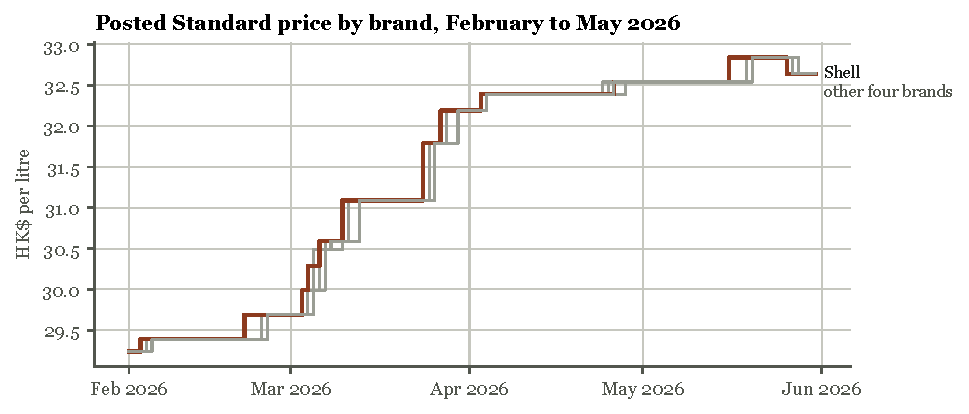
\includegraphics[width=\textwidth]{figures/ex2_hk_steps.pdf}
\caption{Shell moves first, the others follow within days. Posted Standard price by brand, daily.}
\label{fig:steps}
\end{figure}

Alignment was loosest in 2026 (\hkEqualTwentySix\% of days), the year world gasoline prices swung most, and tightest in 2023 (\hkEqualTwentyThree\%). The gaps are the days it takes the followers to catch up.

\subsection{Leaders and followers}

A change episode starts with the first brand to change price and collects each other brand's first change in the same direction within seven days. There were \hkEpisodes{} episodes for Standard petrol. All five brands moved within the week in \hkShareFullWeek\% of them and by exactly the same amount in \hkShareSameSize\% of those. All five moved on the same day in \hkShareSameDay\%. Of the \hkPartial{} episodes that not every brand joined, \hkLone{} were a single brand moving alone; in \hkLoneReversed{} of those the brand went back to its old price within two weeks.

\begin{figure}[H]
\centering
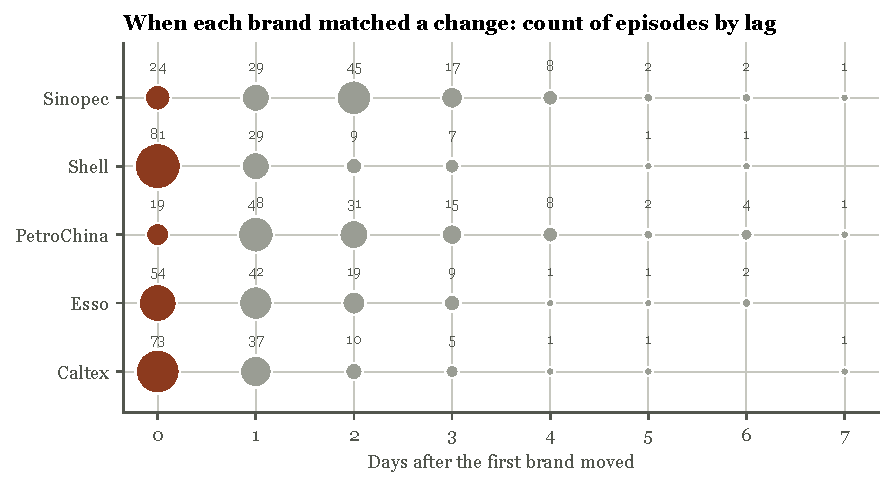
\includegraphics[width=\textwidth]{figures/ex3_hk_lags.pdf}
\caption{Caltex, Shell and Esso are usually first; PetroChina and Sinopec usually follow a day or two later. Number of complete episodes by brand and by days after the first move.}
\label{fig:lags}
\end{figure}

The order is stable (Exhibit~\ref{fig:lags}). When one brand moved alone, it was Shell \hkLeadShell{} times, Esso \hkLeadEsso{} times and Caltex \hkLeadCaltex{} times; PetroChina and Sinopec almost never move first on their own. The premium grade shows the same pattern over a longer span. In January 2024 Shell raised its premium surcharge over Standard from \hk 1.19 to \hk 1.60. The other four held at \hk 1.19 for a year, then moved to \hk 1.60 between 7 and 11 January 2025. Three days later Shell raised its surcharge to \hk 1.80, and all four matched within a week.

\subsection{Rises and cuts}

Of the \hkEpisodes{} episodes, \hkEpisodesUp{} were increases and \hkEpisodesDown{} were cuts. The median increase was \hk\hkSizeUp{} a litre and the median cut \hk\hkSizeDown. In 2023 and 2024 together there were \hkUpTwentyThreeFour{} increases and \hkDownTwentyThreeFour{} cuts. Small, frequent increases and rarer, smaller cuts are a pattern that cost movements alone would not produce: costs fell in those years.

\section{Prices and costs}

\subsection{The margin over cost}

Exhibit~\ref{fig:decomp} splits the monthly posted Standard price into the import cost of the petrol, the fixed duty, and what is left: the margin that pays for storage, distribution, stations, land and profit. In the first twelve months of the sample the posted price averaged \hk\postedFirst{} and the margin \hk\marginFirst. In the twelve months to \marginEnd{} the posted price averaged \hk\postedLast{} and the margin \hk\marginLast. The import cost rose from \hk\importFirst{} to \hk\importLast{} over the same span. Of the \hk\postedRise{} rise in the posted price, \hk\marginRise{} (\marginShareOfRise\%) is margin and \hk\importRise{} is the cost of the petrol.

\begin{figure}[H]
\centering
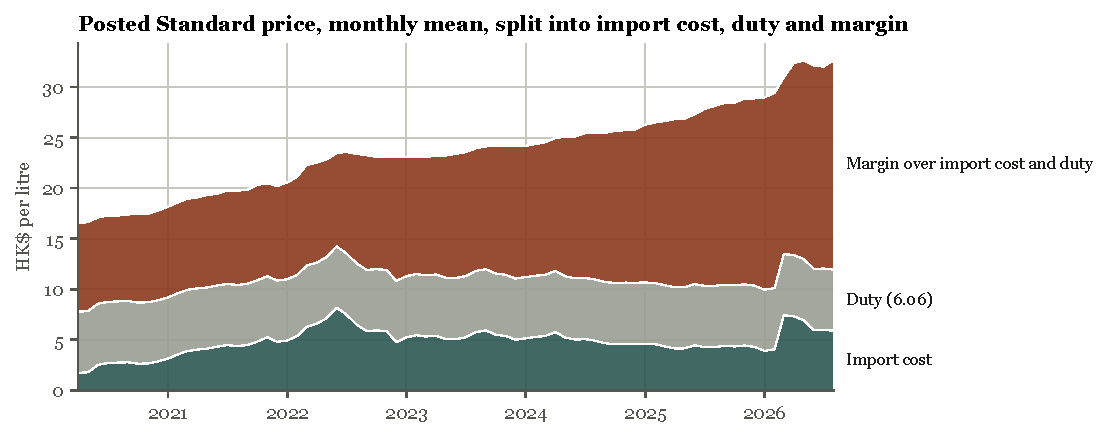
\includegraphics[width=\textwidth]{figures/ex1_hk_decomposition.pdf}
\caption{Most of the rise in the posted price since 2020 is margin. Monthly mean posted Standard price split into import unit value, duty and the remainder.}
\label{fig:decomp}
\end{figure}

The clearest stretch is January 2023 to December 2025. The posted price rose from \hk\spanPostedFrom{} to \hk\spanPostedTo{} while the import cost fell from \hk\spanImportFrom{} to \hk\spanImportTo. Some of the margin pays for costs that rose in those years, rents and wages among them, and this paper has no data on those. It is hard, though, for station operating costs to account for a margin that more than doubled in six years.

\subsection{Discounts}

The posted price is not what most buyers pay. Each brand advertises a walk-in discount for anyone who fills up, and deeper discounts for card and loyalty holders. The Consumer Council's comparison page, archived on \discDays{} days between \discFirst{} and \discLast, shows the walk-in discounts widening as posted prices rose (Exhibit~\ref{fig:disc}). The largest walk-in discount on Standard was \hk\discMaxFirst{} on the first archived day and \hk\discMaxLast{} on the last; the cheapest net price went from \hk\discNetMinFirst{} to \hk\discNetMinLast, against posted prices of \hk\discPumpFirst{} and \hk\discPumpLast.

\begin{figure}[H]
\centering
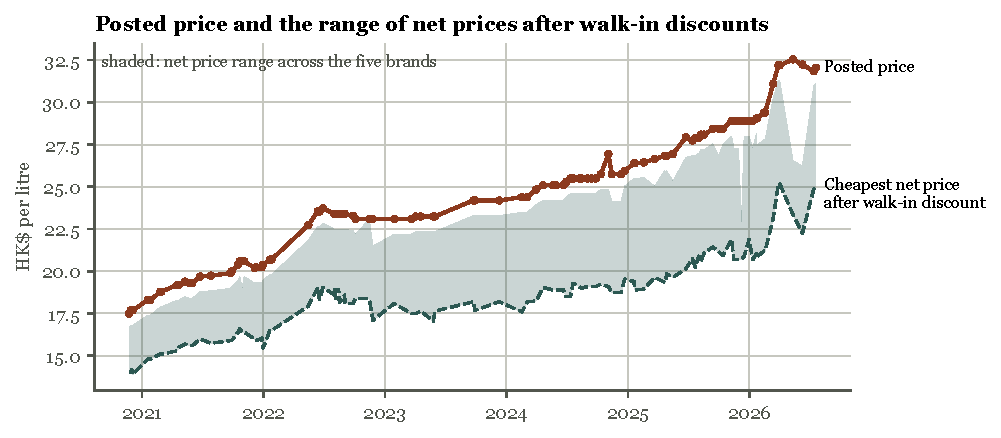
\includegraphics[width=\textwidth]{figures/ex4_hk_discounts.pdf}
\caption{Discounts widened as posted prices rose, but net prices rose too. Posted Standard price and the range of net prices after each brand's walk-in discount, on days the Consumer Council page was archived.}
\label{fig:disc}
\end{figure}

Discounts do not explain the rising margin away. The average walk-in discount across the five brands was \hk\discMeanFirst{} a litre in the first year of archived pages and \hk\discMeanLast{} in the last. Taking the average net price instead of the posted one, the margin over import cost and duty went from \hk\netMarginFirst{} to \hk\netMarginLast, close to the same doubling. Card and loyalty discounts are deeper still and are not observed, so the margin on an average sale is lower than this, and how it changed is unknown.

The discounts do show that brands compete on net price: on any given day they differ widely across brands. But they sit on top of a posted price that does not differ, and the Competition Commission found the discount system ``complex and opaque'' and ``not a perfect substitute for price competition'' \parencite{compcomm2017}.

\subsection{Pass-through}

The standard test for asymmetric pass-through is an error-correction model in which retail price changes respond separately to rises and falls in cost \parencite{bcg1997}. Each market is estimated on weekly data with four lags of cost changes and one lag of the retail change; Hong Kong's long-run relation includes a time trend because its margin drifts upward (about \hk\hkTrendYear{} a litre a year). Exhibit~\ref{fig:pt} shows the simulated response to a permanent one-unit change in cost.

\begin{figure}[H]
\centering
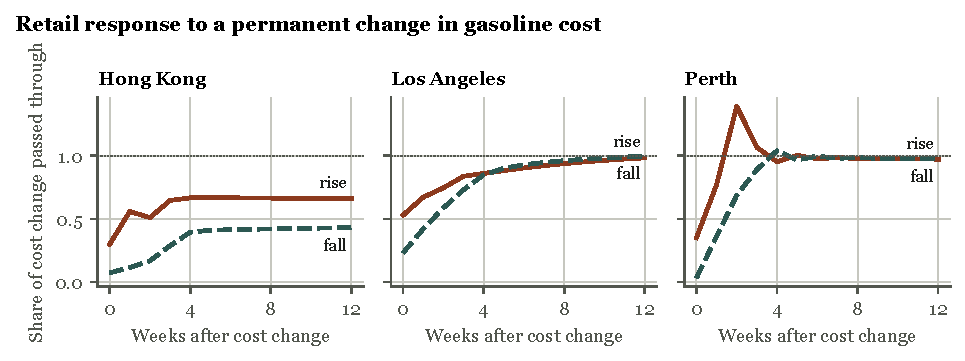
\includegraphics[width=\textwidth]{figures/ex5_passthrough.pdf}
\caption{Hong Kong and Los Angeles pass cost rises through faster than falls; Perth does not, once its weekly cycle is accounted for. Cumulative share of a permanent cost change passed to the retail price.}
\label{fig:pt}
\end{figure}

\begin{table}[H]
\small
\caption{Share of a cost change passed through, by week}
\label{tab:pt}
\begin{tabularx}{\textwidth}{@{}X r r r r r@{}}
\toprule
 & \multicolumn{2}{c}{Week 0} & \multicolumn{2}{c}{Week 4} & Rise = fall, \\
Market & Rise & Fall & Rise & Fall & weeks 0 to 1 ($p$) \\
\midrule
Hong Kong (posted, Monday) & \hkRiseZero\% & \hkFallZero\% & \hkRiseFour\% & \hkFallFour\% & \hkAsymP \\
Los Angeles (EIA weekly) & \laRiseZero\% & \laFallZero\% & \laRiseFour\% & \laFallFour\% & \laAsymP \\
Perth (Tuesday median) & \perthRiseZero\% & \perthFallZero\% & \perthRiseFour\% & \perthFallFour\% & \perthAsymP \\
\bottomrule
\end{tabularx}
\par\smallskip\footnotesize Cost is the Los Angeles RBOB spot price for Los Angeles and the US Gulf Coast spot price in local currency for Hong Kong and Perth. Newey-West standard errors. Results with six and eight lags, and for Perth at the weekly mean and the Wednesday peak, are in \texttt{results/passthrough\_robustness.csv}; the Hong Kong and Los Angeles asymmetries are significant at 5\% in every specification and Perth's in none.
\end{table}

Hong Kong's asymmetry is the largest of the three. Part of it is mechanical: the posted price changed in only \hkUnchangedWeeks\% of weeks, against nearly every week in Los Angeles and Perth, so any lag in adjusting shows up as slow pass-through in both directions. The asymmetry is the part that is not mechanical. Rises are passed on faster than falls, and in the long run less than half of a fall is passed on at all.

\section{The comparison markets}

\textbf{Los Angeles.} Retail prices in Los Angeles track the spot price closely (a correlation in levels above 0.95), change almost every week, and show the familiar ``rockets and feathers'' asymmetry: \laRiseZero\% of a cost rise reaches the pump within the week against \laFallZero\% of a fall, though both are almost fully passed through within three months. The asymmetry is consistent with consumer search costs and is not, by itself, evidence of coordination \parencite{bcg1997}.

\textbf{Perth.} Perth combines complete price transparency with many sellers: about \perthStations{} metropolitan stations under dozens of brands. On a typical day the gap between the cheapest and dearest station is \perthRange{} cents a litre and the interquartile range \perthIqr{} cents. Medians by brand differ by about \perthBrandRange{} cents. Prices follow a weekly cycle in which the major brands restore prices on the same day each week and then undercut each other back down (Exhibit~\ref{fig:perth}). \textcite{byrne2019} show that this cycle is itself a coordination device: over a three-year transition, the dominant firms used price leadership and price experiments to settle the market on a focal weekly pattern. So Perth is no benchmark of pure competition either. What it shows is that full transparency among many sellers ends each week in a synchronized restoration followed by a price war.

\begin{figure}[H]
\centering
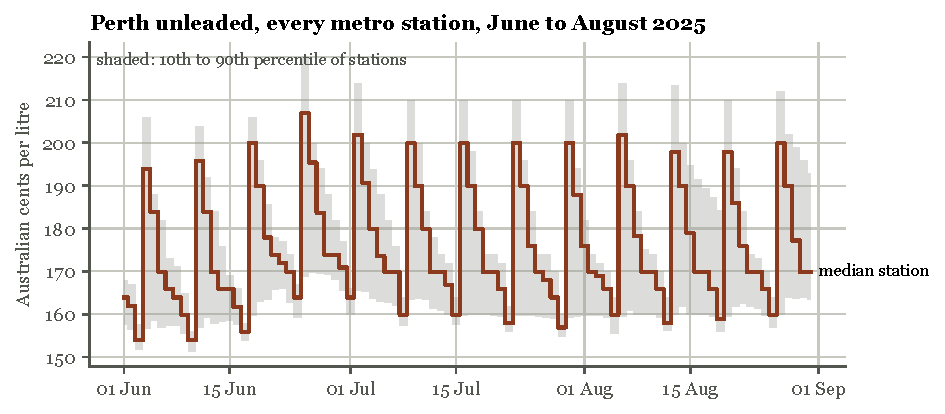
\includegraphics[width=\textwidth]{figures/ex6_perth_cycle.pdf}
\caption{Perth's prices cycle every week and spread widely across stations. Daily median and 10th to 90th percentile of metropolitan unleaded prices.}
\label{fig:perth}
\end{figure}

\section{What the screens can and cannot show}
\label{sec:law}

\textbf{The legal standard.} In the United States, an agreement among competitors to fix prices is unlawful per se.\footnote{\emph{United States v. Socony-Vacuum Oil Co.}, 310 U.S. 150 (1940).} Parallel pricing is not. The Supreme Court has held that ``conscious parallelism'' has ``not yet read conspiracy out of the Sherman Act entirely'',\footnote{\emph{Theatre Enterprises, Inc. v. Paramount Film Distributing Corp.}, 346 U.S. 537, 541 (1954).} but that parallel conduct alone is ``just as much in line with a wide swath of rational and competitive business strategy'' and must be placed ``in a context that raises a suggestion of a preceding agreement''.\footnote{\emph{Bell Atlantic Corp. v. Twombly}, 550 U.S. 544 (2007) (Part II).} Hong Kong's First Conduct Rule, in force since December 2015, prohibits agreements and concerted practices that harm competition.\footnote{Competition Ordinance (Cap. 619) s.~6; the conduct rules came into force on 14 December 2015.} Both regimes require something beyond identical prices.

\textbf{What the evidence here supports.} Each pattern in this paper has an innocent reading. Identical posted prices follow from identical costs and public prices. A stable leader is what a price-leadership equilibrium looks like with or without an agreement. Asymmetric pass-through appears in competitive markets with search costs. A rising margin can reflect rising land and labor costs. What the screens add is that the patterns occur together, persist for six years, and are strongest exactly where cost explanations are weakest: increases with no cuts through two years of falling import costs. In the language of screening, Hong Kong fails the screens that Perth and Los Angeles pass or fail more mildly, and that is a reason to ask for more evidence.

\textbf{What would distinguish the explanations.} Station-level operating costs and land rents would show how much of the margin is cost. The timing of price notices (when each brand tells the Consumer Council of a change, and whether brands learn of each other's changes before the public does) would show whether the leader-follower pattern runs through public information or around it. Walk-in and card discount terms by date, which the Council collects but does not publish as data, would show whether the net prices that customers pay move in lockstep as the posted prices do. The Competition Commission's 2017 study described the follow-within-a-day-or-two pattern documented here and concluded that, on its own, it ``reveals very little about whether firms are competing or coordinating'' \parencite{compcommglance}. It recommended prominent display of pump prices and walk-in discounts, more station sites, and a review of how sites are tendered \parencite{compcomm2017}. The margin in the years since, on posted and on net prices, has roughly doubled.

\section{Limitations}

\begin{itemize}
\item The Hong Kong record starts in April 2020, the first version kept by the open-data archive. Earlier years, including the period of the Commission's study, are not covered.
\item Day-level timing in Hong Kong depends on when the archive harvested the file. A one-day gap between brands may be a harvesting artifact; the leader-follower order across \hkEpisodes{} episodes is not.
\item The import unit value is monthly and averages consignments, so it lags spot prices. The weekly pass-through model uses a world gasoline price that is a different grade from Hong Kong's.
\item The margin is gross. It includes storage, distribution, station costs and rents, none of which are observed.
\item Discounts are observed only on archived days, and card and loyalty discounts are not observed at all.
\end{itemize}

\appendix
\section{Method notes}

\textbf{Episodes.} For each grade, a change is any day on which a brand's posted price differs from the day before. Changes are processed in date order; an episode opens with the earliest unassigned change and collects, for each brand, its first unassigned change in the same direction within seven days. Lags are measured in days from the opening change.

\textbf{Pass-through model.} For retail price $r_t$ and cost $x_t$ in the same units, the long-run relation $r_t = c + \theta x_t\ (+\ \delta t)$ is estimated in levels, and the short-run model is
\[
\Delta r_t = a + \sum_{k=0}^{4} \left(\beta_k^{+}\Delta x^{+}_{t-k} + \beta_k^{-}\Delta x^{-}_{t-k}\right) + \phi\,\Delta r_{t-1} + \gamma\,(r_{t-1} - \hat c - \hat\theta x_{t-1} - \hat\delta (t-1)) + \varepsilon_t,
\]
where $\Delta x^{+}$ keeps cost rises and $\Delta x^{-}$ keeps cost falls. Responses are simulated from the fitted coefficients for a permanent unit step. The asymmetry test is a Wald test that $\beta_0^{+}+\beta_1^{+} = \beta_0^{-}+\beta_1^{-}$, with Newey-West standard errors.

\textbf{Data decisions} are listed in \texttt{docs/decisions.md} in the repository, including the treatment of one-snapshot reporting faults in the premium series and the choice of Perth's Tuesday price.

\printbibliography[title=References]

\end{document}
